%========================================================
% Lecture Notes (LaTeX) — Fluids: Density, Pressure, Pascal, Atmosphere
% High-quality colored diagrams with TikZ
%========================================================
\documentclass[11pt]{article}

\usepackage[margin=1in]{geometry}
\usepackage{amsmath, amssymb}
\usepackage{siunitx}
\usepackage{physics}
\usepackage{graphicx}
\usepackage{microtype}
\usepackage{xcolor}
\usepackage{tcolorbox}
\usepackage{tikz}
\usetikzlibrary{arrows.meta, calc, patterns, positioning, decorations.pathreplacing}

%------------------------
% Color palette (soft + professional)
%------------------------
\definecolor{Accent}{HTML}{B21F3A}     % deep red (headings)
\definecolor{Ink}{HTML}{1D2433}        % near-black
\definecolor{Steel}{HTML}{2D5D7B}      % blue
\definecolor{FluidBlue}{HTML}{4FA3D1}  % water
\definecolor{FluidOil}{HTML}{D9A441}   % oil
\definecolor{Mercury}{HTML}{8D8D8D}    % mercury (gray)
\definecolor{Light}{HTML}{F6F7FB}      % background tint
\definecolor{Rule}{HTML}{D8DCE6}       % light rule lines

\setlength{\parindent}{0pt}
\setlength{\parskip}{8pt}

\sisetup{
  detect-all,
  per-mode=symbol,
  exponent-product=\cdot
}

%------------------------
% Boxes
%------------------------
\tcbset{
  colback=Light,
  colframe=Rule,
  arc=2mm,
  boxrule=0.6pt,
  left=10pt,right=10pt,top=8pt,bottom=8pt
}

\newtcolorbox{keybox}[1]{
  title=\textcolor{Accent}{\bfseries #1},
  colback=Light,
  colframe=Rule
}

%------------------------
% TikZ styles
%------------------------
\tikzset{
  axis/.style={-Latex, line width=0.9pt, color=Ink},
  dim/.style={Latex-Latex, line width=0.9pt, color=Ink},
  force/.style={-Latex, line width=1.1pt, color=Accent},
  label/.style={color=Ink, font=\small},
  water/.style={fill=FluidBlue, fill opacity=0.30, draw=Steel, line width=0.9pt},
  oil/.style={fill=FluidOil, fill opacity=0.35, draw=Steel, line width=0.9pt},
  mercury/.style={fill=Mercury, fill opacity=0.35, draw=Steel, line width=0.9pt},
  vessel/.style={draw=Ink, line width=1.0pt, rounded corners=1.5pt},
  dashedguide/.style={dash pattern=on 2pt off 2pt, color=Ink!45, line width=0.8pt},
}

%========================================================
\begin{document}

{\Large \bfseries \textcolor{Accent}{Day 1 — Week 4 \quad Chapter 13: Fluids and Density}}\\[-2pt]
\rule{\textwidth}{0.6pt}

%========================================================
\section*{\textcolor{Accent}{13.1 Fluids and Density}}

\begin{keybox}{What is a fluid?}
\textbf{Fluids} are materials that \textbf{flow}: they deform continuously under shear stress.
\begin{itemize}
  \item \textbf{Gases and liquids} are fluids.
  \item Many introductory problems treat liquids as \textbf{incompressible}: their density is approximately constant.
\end{itemize}
\end{keybox}

\begin{keybox}{Compressibility (idea)}
For an \textbf{incompressible} fluid, density does not change appreciably with pressure:
\[
\Delta \rho \approx 0 \quad \text{even if} \quad \Delta P \neq 0.
\]
(Real fluids compress slightly, but often the effect is negligible for liquids.)
\end{keybox}

%------------------------
% Diagram: gas vs liquid packing
%------------------------
\begin{center}
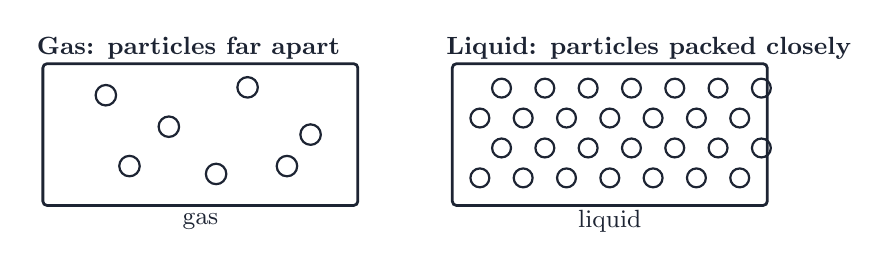
\begin{tikzpicture}[scale=1.0]
  % Gas box
  \node[label, anchor=west] at (-0.2,2.2) {\textbf{Gas: particles far apart}};
  \draw[vessel] (0,0.2) rectangle (4,2.0);
  \foreach \p in {(0.8,1.6),(1.6,1.2),(2.6,1.7),(3.4,1.1),(1.1,0.7),(2.2,0.6),(3.1,0.7)}{
    \draw[Ink, line width=0.8pt] \p circle (0.13);
  }
  \node[label] at (2,0.0) {gas};

  % Liquid box
  \node[label, anchor=west] at (5.0,2.2) {\textbf{Liquid: particles packed closely}};
  \draw[vessel] (5.2,0.2) rectangle (9.2,2.0);
  % Packed circles
  \foreach \i in {0,...,6}{
    \foreach \j in {0,...,3}{
      \pgfmathsetmacro\x{5.55 + 0.55*\i + 0.275*mod(\j,2)}
      \pgfmathsetmacro\y{0.55 + 0.38*\j}
      \draw[Ink, line width=0.8pt] (\x,\y) circle (0.12);
    }
  }
  \node[label] at (7.2,0.0) {liquid};
\end{tikzpicture}
\end{center}

%========================================================
\subsection*{\textcolor{Accent}{Density}}

\begin{keybox}{Definition}
\[
\rho \equiv \frac{m}{V},
\qquad\text{so}\qquad
m=\rho V.
\]
If $\rho$ is constant (incompressible), then $m \propto V$.
\end{keybox}

\begin{keybox}{Unit conversion example (water)}
Water has density approximately
\[
\rho_{\text{water}} \approx \SI{1}{g/cm^3} = \SI{1000}{kg/m^3}.
\]
Therefore, $1~\si{m^3}$ of water has mass $\approx \SI{1000}{kg}$.
\end{keybox}

%------------------------
% Diagram: linear m vs V
%------------------------
\begin{center}
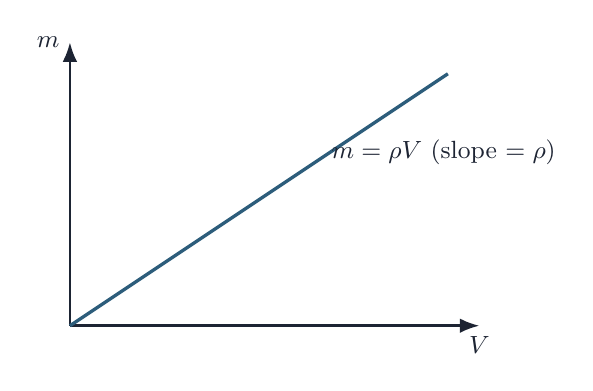
\begin{tikzpicture}[scale=1.0]
  \draw[axis] (0,0) -- (5.2,0) node[below,label] {$V$};
  \draw[axis] (0,0) -- (0,3.6) node[left,label] {$m$};
  \draw[Steel, line width=1.2pt] (0,0) -- (4.8,3.2);
  \node[label, anchor=west] at (3.2,2.2) {$m=\rho V$ (slope $=\rho$)};
\end{tikzpicture}
\end{center}

%========================================================
\section*{\textcolor{Accent}{Pressure}}

\begin{keybox}{Definition}
\[
P \equiv \frac{F}{A}.
\]
SI units:
\[
\SI{1}{Pa} = \SI{1}{N/m^2} = \SI{1}{kg\,m^{-1}\,s^{-2}}.
\]
\end{keybox}

%------------------------
% Diagram: force on piston and side holes (pressure same at depth)
%------------------------
\begin{center}
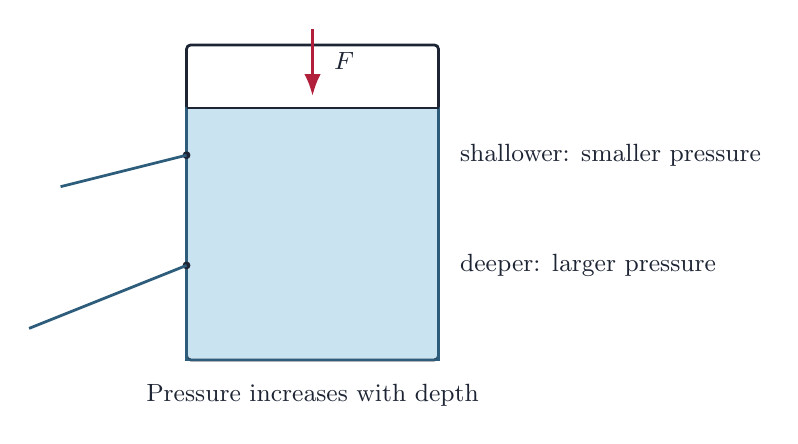
\begin{tikzpicture}[scale=1.0]
  % Container
  \draw[vessel] (0,0) rectangle (3.2,4.0);

  % Fluid fill
  \draw[water] (0,0) rectangle (3.2,3.2);

  % Piston plate
  \draw[Ink, line width=1.0pt] (0,3.2) -- (3.2,3.2);

  % Force arrow
  \draw[force] (1.6,4.2) -- (1.6,3.35);
  \node[label, anchor=west] at (1.75,3.8) {$F$};

  % Holes and jets (two depths)
  \fill[Ink] (0,2.6) circle (0.05);
  \fill[Ink] (0,1.2) circle (0.05);
  \draw[Steel, line width=1.0pt] (0,2.6) -- (-1.6,2.2);
  \draw[Steel, line width=1.0pt] (0,1.2) -- (-2.0,0.4);

  \node[label, anchor=west] at (3.35,2.6) {shallower: smaller pressure};
  \node[label, anchor=west] at (3.35,1.2) {deeper: larger pressure};

  \node[label] at (1.6,-0.45) {Pressure increases with depth};
\end{tikzpicture}
\end{center}

\begin{keybox}{Key idea: pressure in a static fluid}
In a fluid at rest, pressure depends mainly on \textbf{depth} (and density), not on horizontal position.
\end{keybox}

%========================================================
\section*{\textcolor{Accent}{Hydrostatic Pressure (Pressure vs. Depth)}}

\begin{keybox}{Result}
At depth $d$ below the surface of a fluid open to the atmosphere,
\[
P = P_0 + \rho g d,
\]
where $P_0$ is the pressure at the surface (often $P_{\text{atm}}$).
\end{keybox}

\begin{keybox}{Quick derivation (force balance on a fluid column)}
Consider a vertical column of fluid of cross-sectional area $A$ and height $d$.
\[
\sum F_y = 0
\quad\Rightarrow\quad
P_{\text{bottom}}A - P_0A - mg = 0.
\]
With $m=\rho V=\rho(Ad)$, we get
\[
P_{\text{bottom}} = P_0 + \rho g d.
\]
\end{keybox}

%------------------------
% Diagram: fluid column force balance
%------------------------
\begin{center}
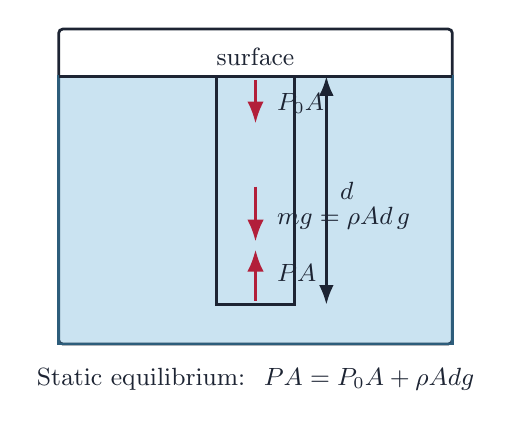
\begin{tikzpicture}[scale=1.0]
  % Fluid region outline
  \draw[vessel] (0,0) rectangle (5.0,4.0);
  \draw[water] (0,0) rectangle (5.0,3.4);
  \draw[Ink, line width=1.0pt] (0,3.4) -- (5.0,3.4);

  % Column
  \draw[Ink, line width=1.0pt] (2.0,0.5) rectangle (3.0,3.4);
  \node[label] at (2.5,3.65) {surface};

  % Depth d
  \draw[dim] (3.4,3.4) -- (3.4,0.5);
  \node[label, anchor=west] at (3.45,1.95) {$d$};

  % Forces
  \draw[force] (2.5,3.35) -- (2.5,2.8);
  \node[label, anchor=west] at (2.65,3.05) {$P_0A$};

  \draw[force] (2.5,0.55) -- (2.5,1.2);
  \node[label, anchor=west] at (2.65,0.9) {$P A$};

  \draw[force] (2.5,2.0) -- (2.5,1.3);
  \node[label, anchor=west] at (2.65,1.6) {$mg=\rho Ad\,g$};

  \node[label] at (2.5,-0.45) {Static equilibrium: $\;PA = P_0A + \rho Ad g$};
\end{tikzpicture}
\end{center}

%========================================================
\section*{\textcolor{Accent}{Pascal’s Principle}}

\begin{keybox}{Statement}
If an \textbf{external pressure increase} $\Delta P$ is applied to a confined fluid, that increase is transmitted
\textbf{undiminished} to \textbf{all points} in the fluid and to the container walls.
\end{keybox}

%------------------------
% Diagram: Pascal principle (push on piston)
%------------------------
\begin{center}
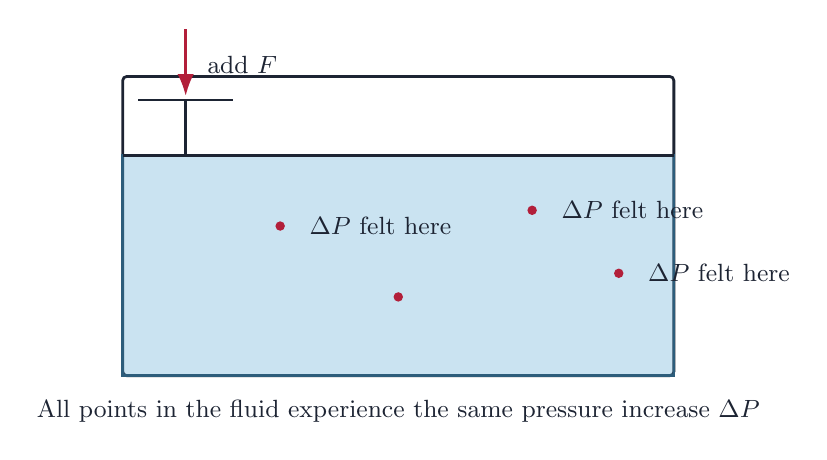
\begin{tikzpicture}[scale=1.0]
  \draw[vessel] (0,0) rectangle (7.0,3.8);
  \draw[water] (0,0) rectangle (7.0,2.8);
  \draw[Ink, line width=1.0pt] (0,2.8) -- (7.0,2.8);

  % Piston at left
  \draw[Ink, line width=1.0pt] (0.8,2.8) -- (0.8,3.5);
  \draw[Ink, line width=1.0pt] (0.2,3.5) -- (1.4,3.5);

  \draw[force] (0.8,4.4) -- (0.8,3.55);
  \node[label, anchor=west] at (0.95,3.95) {add $F$};

  % Dots indicating points in fluid
  \foreach \p in {(2.0,1.9),(3.5,1.0),(5.2,2.1),(6.3,1.3)}{
    \fill[Accent] \p circle (0.06);
  }

  % Labels
  \node[label, anchor=west] at (2.25,1.9) {$\Delta P$ felt here};
  \node[label, anchor=west] at (5.45,2.1) {$\Delta P$ felt here};
  \node[label, anchor=west] at (6.55,1.3) {$\Delta P$ felt here};

  \node[label] at (3.5,-0.45) {All points in the fluid experience the same pressure increase $\Delta P$};
\end{tikzpicture}
\end{center}

%========================================================
\section*{\textcolor{Accent}{Example: Pressure at a Point in a Connected Fluid}}

\begin{keybox}{Setup}
A static fluid open to the atmosphere: pressure at depth $d$ is
\[
P = P_{\text{atm}} + \rho g d.
\]
Only the \textbf{vertical depth} below the free surface matters (not the shape of the container).
\end{keybox}

%------------------------
% Diagram: connected container with two surface heights (100 cm vs 40 cm idea)
%------------------------
% \begin{center}
% \begin{tikzpicture}[scale=1.0]
%   % Left container (tall)
%   \draw[vessel] (0,0) -- (0,3.8) -- (1.2,3.8) -- (1.2,1.4) -- (3.2,1.4) -- (3.2,3.0) -- (4.4,3.0) -- (4.4,0) -- cycle;
%   \draw[water] (0.02,0.02) -- (0.02,3.2) -- (1.18,3.2) -- (1.18,1.42) -- (3.22,1.42) -- (3.22,2.4) -- (4.38,2.4) -- (4.38,0.02) -- cycle;

%   % Free surfaces
%   \draw[Ink, line width=1.0pt] (0.02,3.2) -- (1.18,3.2);
%   \draw[Ink, line width=1.0pt] (3.22,2.4) -- (4.38,2.4);

%   % Mark point on right bottom region
%   \fill[Accent] (3.7,1.0) circle (0.07);
%   \node[label, anchor=west] at (3.85,1.0) {$P=?$};

%   % Heights markers
%   \draw[dim] (-0.6,3.2) -- (-0.6,0.2);
%   \node[label, anchor=west] at (-0.55,1.7) {\SI{100}{cm}};

%   \draw[dim] (5.0,2.4) -- (5.0,0.2);
%   \node[label, anchor=west] at (5.05,1.3) {\SI{40}{cm}};

%   \node[label] at (2.2,-0.45) {Same fluid, different surface heights; pressure depends on depth below the \emph{local} surface.};
% \end{tikzpicture}
% \end{center}

\begin{keybox}{Numerical example (illustrative)}
If $d=\SI{0.60}{m}$ below the water surface and $\rho=\SI{1000}{kg/m^3}$, $g=\SI{9.8}{m/s^2}$:
\[
P \approx P_{\text{atm}} + (1000)(9.8)(0.60)
\approx \SI{1.0e5}{Pa} + \SI{5.9e3}{Pa}
\approx \SI{1.06e5}{Pa}.
\]
\end{keybox}

%========================================================
\section*{\textcolor{Accent}{Atmospheric Pressure}}

\begin{keybox}{Basic facts}
\begin{itemize}
  \item Atmospheric pressure generally \textbf{decreases with altitude}.
  \item Air tends to flow from \textbf{high pressure} to \textbf{low pressure}.
  \item Weather connection (qualitative): low pressure is often associated with stormy conditions; high pressure often with clearer weather.
\end{itemize}
\end{keybox}

%------------------------
% Diagram: pressure vs altitude (qualitative)
%------------------------
\begin{center}
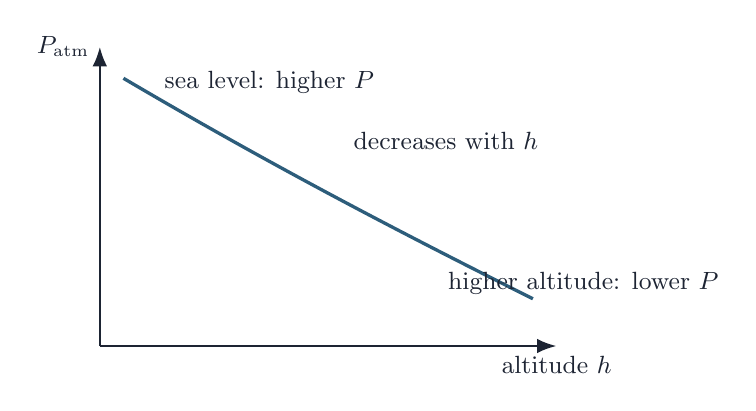
\begin{tikzpicture}[scale=1.0]
  \draw[axis] (0,0) -- (5.8,0) node[below,label] {altitude $h$};
  \draw[axis] (0,0) -- (0,3.8) node[left,label] {$P_{\text{atm}}$};
  \draw[Steel, line width=1.2pt] (0.3,3.4) .. controls (2.0,2.4) and (3.5,1.6) .. (5.5,0.6);
  \node[label, anchor=west] at (3.1,2.6) {decreases with $h$};

  \node[label, anchor=west] at (0.7,3.35) {sea level: higher $P$};
  \node[label, anchor=west] at (4.3,0.8) {higher altitude: lower $P$};
\end{tikzpicture}
\end{center}

%========================================================
\section*{\textcolor{Accent}{Barometer (Mercury Column)}}

\begin{keybox}{Concept}
A mercury barometer balances atmospheric pressure with the hydrostatic pressure of a mercury column:
\[
P_{\text{atm}} = \rho_{\text{Hg}} g h.
\]
\end{keybox}

%------------------------
% Diagram: mercury barometer
%------------------------
\begin{center}
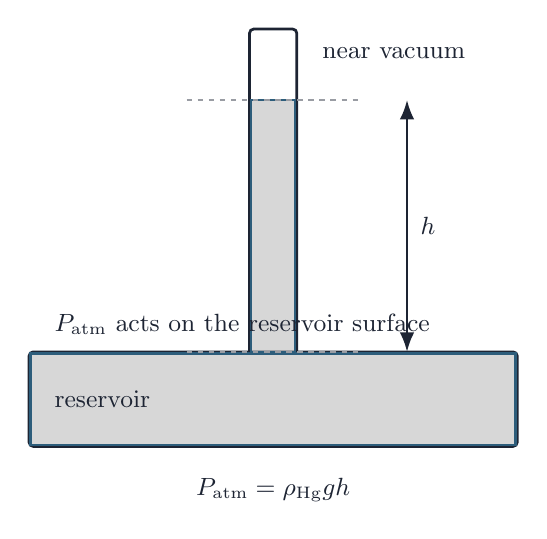
\begin{tikzpicture}[scale=1.0]
  % Reservoir
  \draw[vessel] (0,0) rectangle (6.2,1.2);
  \draw[mercury] (0.02,0.02) rectangle (6.18,1.18);

  % Tube
  \draw[vessel] (2.8,1.2) -- (2.8,5.3) -- (3.4,5.3) -- (3.4,1.2);
  % Mercury column in tube
  \draw[mercury] (2.82,1.2) rectangle (3.38,4.4);

  % Vacuum at top
  \node[label, anchor=west] at (3.6,5.0) {near vacuum};

  % Mark heights
  \draw[dashedguide] (2.0,4.4) -- (4.2,4.4);
  \draw[dashedguide] (2.0,1.2) -- (4.2,1.2);
  \draw[dim] (4.8,4.4) -- (4.8,1.2);
  \node[label, anchor=west] at (4.85,2.8) {$h$};

  % Labels
  \node[label, anchor=west] at (0.2,0.6) {reservoir};
  \node[label, anchor=west] at (0.2,1.55) {$P_{\text{atm}}$ acts on the reservoir surface};

  \node[label] at (3.1,-0.55) {$P_{\text{atm}}=\rho_{\text{Hg}}gh$};
\end{tikzpicture}
\end{center}

\begin{keybox}{Typical value}
With $\rho_{\text{Hg}}\approx \SI{13600}{kg/m^3}$ and $P_{\text{atm}}\approx \SI{1.01e5}{Pa}$,
\[
h \approx \frac{P_{\text{atm}}}{\rho_{\text{Hg}}g} \approx \SI{0.76}{m} \approx \SI{76}{cm}.
\]
\end{keybox}

%========================================================
\section*{\textcolor{Accent}{Manometers (U-tubes)}}

\begin{keybox}{Rule for static connected fluids}
At the \textbf{same horizontal level} in the \textbf{same connected fluid}, pressures are equal.
\end{keybox}


\end{document}
